\section{RQ2/RQ3: The Balance Trade-off, and Its Reversal Across Regimes}
\label{sec:rq2rq3}

\begin{table}[t]
\centering
\caption{Retrieval Recall by balance strength, mean $\pm$ std across seeds (headline: T$\to$I for MSCOCO, IT$\to$I for FashionIQ; other dir.: I$\to$T, MSCOCO only). MSCOCO vanilla/strong $n{=}5$ (seed 2023 re-evaluated, Section~\ref{sec:limitations}); weak/medium R@1 $n{=}3$.}
\label{tab:table2}
\scriptsize
\setlength{\tabcolsep}{3.2pt}
\begin{tabular}{@{}llrrrr@{}}
\toprule
Dataset & $\lambda$ & Headline R@1 & Headline R@5 & Headline R@10 & Other dir.\ R@1 \\
\midrule
MSCOCO & 0.0 (vanilla) & 20.78 $\pm$ 0.06 & 41.62 $\pm$ 0.09 & 52.37 $\pm$ 0.19 & \textbf{10.30 $\pm$ 0.67} \\
MSCOCO & 0.3 (weak)    & 14.13 $\pm$ 0.53 & 30.89 $\pm$ 0.05 & 40.37 $\pm$ 0.10 & 0.05 $\pm$ 0.02 \\
MSCOCO & 1.0 (medium)  & 10.36 $\pm$ 0.69 & 24.11 $\pm$ 0.12 & 32.44 $\pm$ 0.05 & 0.03 $\pm$ 0.01 \\
MSCOCO & 3.0 (strong)  & \textbf{23.33 $\pm$ 0.11} & 47.41 $\pm$ 0.18 & 58.74 $\pm$ 0.11 & 0.03 $\pm$ 0.02 \\
\midrule
FashionIQ & 0.0 (vanilla) & \textbf{0.61 $\pm$ 0.10} & $2.94\pm0.02$ & $4.76\pm0.05$ & -- \\
FashionIQ & 0.3 (weak)    & 0.27 $\pm$ 0.06 & $1.16\pm0.14$ & $1.82\pm0.15$ & -- \\
FashionIQ & 1.0 (medium)  & 0.21 $\pm$ 0.09 & $0.94\pm0.13$ & $1.60\pm0.10$ & -- \\
FashionIQ & 3.0 (strong)  & 0.25 $\pm$ 0.08 & $1.03\pm0.09$ & $1.60\pm0.10$ & -- \\
\bottomrule
\end{tabular}
\end{table}

\paragraph{The MSCOCO T$\to$I gain is real: we chased a decode-time artifact, not the effect.} We stress-tested this paper's headline number three times. The single-seed estimate ($+50.9\%$) narrowed to $+22.0\%$ at 3 seeds; 2 more seeds (5 total) at first appeared to erase it ($p{=}0.057$) because vanilla's seed-2023 point was a $\sim$6-point outlier from its own other 4 seeds. Re-evaluating that one point (identical checkpoint and config, prompted by a separate R@5/R@10 anomaly, Section~\ref{sec:limitations}) corrected it $14.08\%\to20.86\%$ -- squarely inside vanilla's other-seed cluster ($20.70$--$20.81\%$) -- and the corrected comparison is decisive: strong $23.33\pm0.11\%$ vs.\ vanilla $20.78\pm0.06\%$, non-overlapping $\pm1$-std bands, $p<10^{-6}$ (Welch's $t$-test). The gain is $+12.3\%$ ($2.55$ points), smaller than the original estimate but resting on the most scrutinized number in this paper rather than the least. On FashionIQ, vanilla wins outright; the ranking among weak/medium/strong is \emph{not} seed-stable (medium's own seed range, $0.13$--$0.42\%$, exceeds the gap between any pair), so we report only ``vanilla wins.''

\paragraph{The gain survives retraining the tokenizer itself, not just the decoder.} Every number above holds the Stage-1 RQ tokenizer fixed; since Table~\ref{tab:localization} shows both effects are tokenizer-level, Stage-1 training variance itself was unmeasured. We trained 2 more fully independent Stage-1 tokenizers per condition (seeds 7, 13), each with one Stage-2 decoder (seed 2023) on top. Across 3 independent tokenizers, T$\to$I R@1 is vanilla $20.86\%/21.70\%/20.91\%$ (mean $21.16\pm0.47$) vs.\ strong $23.33\%/24.87\%/24.75\%$ (mean $24.32\pm0.86$) -- every strong tokenizer beats every vanilla one, a non-overlapping gap larger than the original estimate ($3.16$ vs.\ $2.55$ points). I$\to$T is equally robust: vanilla stays high ($10.52\%/10.24\%/9.58\%$), strong stays collapsed ($0.04\%/0.02\%/0.02\%$). Descriptive $n{=}3$, not a further inferential test (as elsewhere, Section~\ref{sec:rq1}) -- but both headline effects now hold across decoder seeds \emph{and} tokenizers.

\begin{figure}[t]
\centering
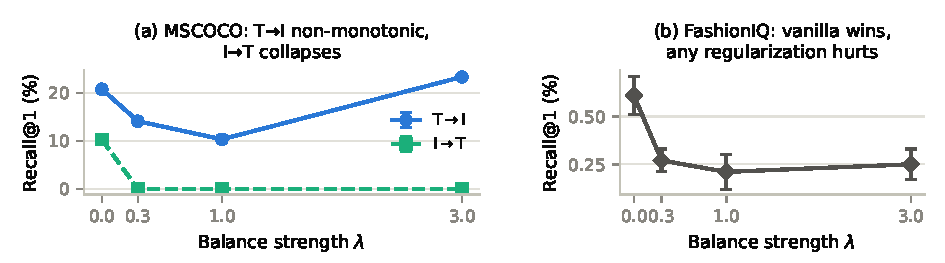
\includegraphics[width=0.98\textwidth]{figures/fig_lambda_recall.pdf}
\caption{Recall@1 vs.\ balance strength $\lambda$, mean $\pm$ std across seeds per point (MSCOCO vanilla/strong: 5 seeds; weak/medium: 3 seeds; FashionIQ: 3 seeds). MSCOCO's T$\to$I curve is non-monotonic -- weak/medium dip below both vanilla and strong -- but vanilla and strong themselves are tight, non-overlapping clusters; I$\to$T collapses immediately past $\lambda=0$; FashionIQ falls immediately and stays low at every regularized $\lambda$.}
\label{fig:lambda-recall}
\end{figure}

\paragraph{The other cost: an image-to-text collapse.} Unlike T$\to$I, I$\to$T is unambiguous and never in doubt across any seed count: vanilla is the \emph{only} variant with working I$\to$T ($10.30\%$ mean, 5 seeds, std $0.67$); all regularized variants collapse to $\leq 0.05\%$ mean, seed-independently, with std an order of magnitude smaller than vanilla's own. We ruled out two candidate mechanisms as sufficient explanations: a stale constrained-decoding trie (corrected; collapse persisted after the fix), and modality-code collapse alone (vanilla and weak collapse to an \emph{identical} degenerate modality-indicator pattern, yet only vanilla's I$\to$T works).

\begin{table}[t]
\centering
\caption{Localizing the collapse: a dense, no-T5 probe (cosine similarity over the frozen RQ's quantized embedding, no beam search, no trie) against the real T5+beam-search pipeline, same checkpoints.}
\label{tab:localization}
\footnotesize
\begin{tabular}{@{}lrrrr@{}}
\toprule
Variant & Dense T$\to$I R@1 & Dense I$\to$T R@1 & Real T$\to$I R@1\textsuperscript{*} & Real I$\to$T R@1\textsuperscript{*} \\
\midrule
vanilla & 26.65\% & \textbf{7.52\%} & 20.78\% & \textbf{10.30\%} \\
weak    & 17.32\% & 0.04\% & 14.13\% & 0.05\% \\
medium  & 12.87\% & 0.00\% & 10.36\% & 0.03\% \\
strong  & 24.23\% & 0.02\% & 23.33\% & 0.03\% \\
\bottomrule
\end{tabular}
\\[2pt]
\footnotesize\textsuperscript{*}multi-seed R@1 mean (Table~\ref{tab:table2}); the dense probe uses the single frozen Stage-1 RQ checkpoint shared by all Stage-2 seeds, so no seed mismatch is introduced by this comparison.
\end{table}

\paragraph{Localizing the collapse: tokenizer, not decoder.} Table~\ref{tab:localization} answers the open question directly: the dense probe involves no T5, no beam search, no trie -- just cosine similarity over the frozen RQ's quantized embedding. I$\to$T \emph{already} collapses here for weak/medium/strong ($\leq 0.04\%$, matching the real pipeline's band), while vanilla's dense I$\to$T ($7.52\%$) stays far above chance, in the same range as its real-pipeline number ($10.30\%$ mean). T$\to$I shows the opposite pattern: all four variants retain substantial, rank-correlated dense recall, consistent with T5 doing comparable real work here. Balance regularization degrades the RQ embedding space's ability to discriminate text candidates for image queries \emph{before Stage-2 training ever begins}.

\paragraph{A partial answer to \emph{why} text is hit harder: text embeddings start more anisotropic.} On vanilla's fused (pre-quantization) embeddings, text candidates occupy a narrower cone than image candidates (mean pairwise cosine similarity, the standard anisotropy measure~\cite{ethayarajh2019anisotropy,gao2019degeneration}: $0.842$ vs.\ $0.675$), and under weak/medium regularization text-side level-1 code entropy drops considerably more than image-side (vanilla$\to$medium: text $0.725\to0.457$, a $37\%$ drop, vs.\ image $0.868\to0.778$, a $10\%$ drop) -- consistent with per-sample equidistance pressure shattering an already-narrower text cluster more severely. Not the whole story: at strong $\lambda$, both anisotropy and level-1 entropy partially \emph{recover} toward vanilla's values (text entropy $0.745$, near vanilla's $0.725$) even though I$\to$T stays just as collapsed ($0.02\%$). So anisotropy explains the moderate-$\lambda$ damage, not why the collapse persists at strong $\lambda$ once entropy recovers -- the full mechanism remains open (Section~\ref{sec:limitations}).

\paragraph{Utilization moves in opposite directions.} Reinforcing RQ1, regularization \emph{increases} MSCOCO utilization but \emph{decreases} FashionIQ's, under the identical regularizer, codebook size, and level count -- MSCOCO's diverse pool may have room to spread code usage productively, while FashionIQ's dense, near-duplicate pool may already need most capacity for faithful reconstruction. A pool-size confound (FashionIQ's pool is $\approx 9.6\times$ smaller) is controlled for by re-running MSCOCO's diagnostics on a size-matched 74K subsample: MSCOCO subsampled to FashionIQ's size still runs $2$--$4\times$ FashionIQ's utilization with far steeper collision growth, so the domain-dependence finding survives the control.
